\documentclass{article}

\usepackage[margin=1in]{geometry}
\usepackage{tikz}
    \tikzstyle{hollow node} = [circle,draw,inner sep=1.5]
    \tikzstyle{solid node}  = [circle,draw,inner sep=1.5,fill=black]
    \usetikzlibrary{calc}
\usepackage{sgame}
    \gamemathtrue

\author{Damien Prieur}
\title{Problem Set 1 \\ ECON 250}
\date{}

\begin{document}

\maketitle

\section*{Question 1) 2.2}
Consider the following strategic situation concerning the owner of a firm (O), the manager of the firm (M), and a potential worker (W).
The owner first decides whether to hire the worker, to refuse to hire the worker, or to let the manager make the decision.
If the owner lets the manager make the decision, then the manager must choose between hiring the worker or not hiring the worker.
If the worker is hired, then he or she chooses between working diligently and shirking.
Assume that the worker does not know whether he or she was hired by the manager or the owner when he or she makes this decision.
If the worker is not hired, then all three players get a payoff of 0.
If the worker is hired and shirks, then the owner and manger each get a payoff of -1, whereas the worker gets 1.
If the worker is hired by the owner and works diligently, then the owner gets a payoff of 1, the manager gets 0, and the worker gets 0.
If the worker is hired by the manager and works diligently, then the owner gets 0, the manager gets 1, and the worker gets 1.
Represent this game in the extensive form (draw the game tree).
\\

\begin{center}
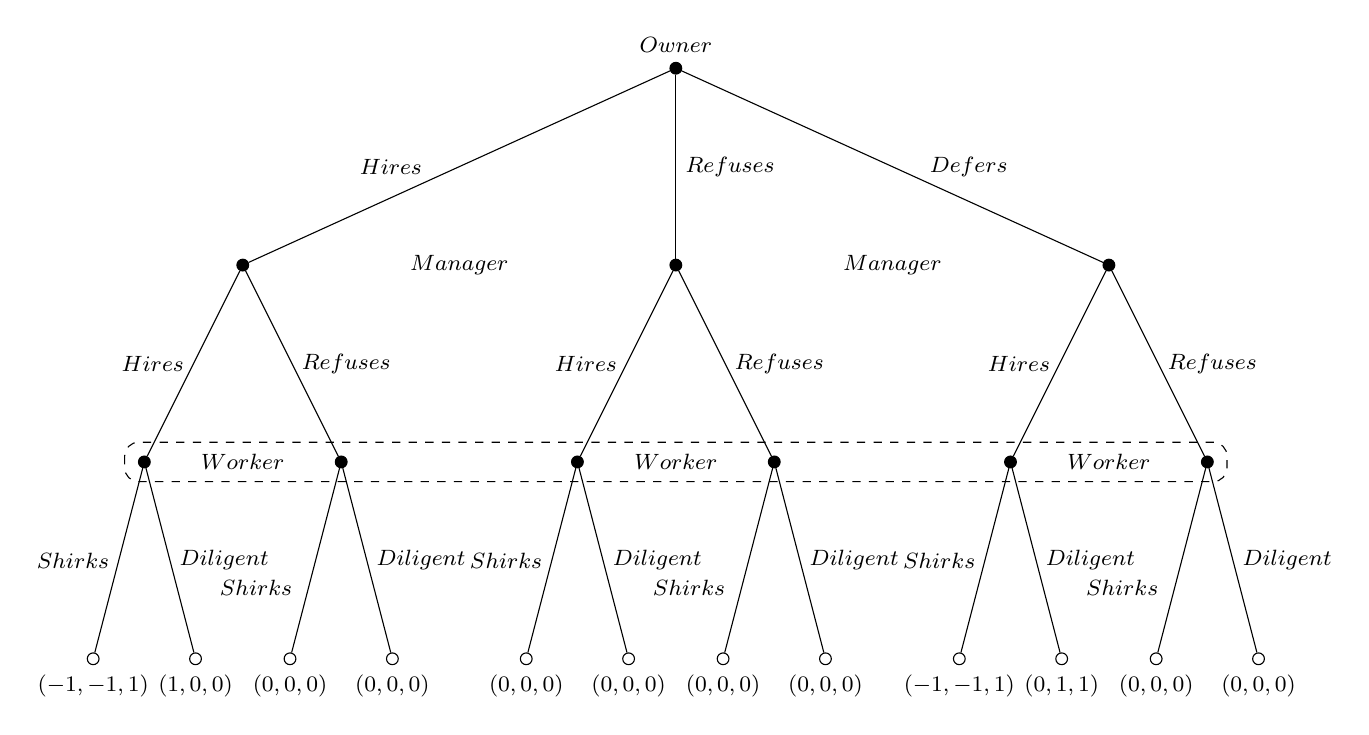
\begin{tikzpicture}[font=\footnotesize]
    \tikzstyle{level 1}=[level distance=25mm, sibling distance=55mm]
    \tikzstyle{level 2}=[level distance=25mm, sibling distance=25mm]
    \tikzstyle{level 3}=[level distance=25mm, sibling distance=13mm]

    % Owner decision
    \node(0)[solid node, label=above:{$Owner$}]{}
        % Manager decision (Owner Hires)
        child{node(1)[solid node]{}
            % Worker Decision (Manager Hires and Owner Hires)
            child{node[solid node]{}
                % Payoffs
                child{node[hollow node, label=below:{$(-1,-1,1)$}]{} edge from parent node[left]{$Shirks$}}
                child{node[hollow node, label=below:{$(1,0,0)$}]{} edge from parent node[right]{$Diligent$}}
                % Manager Hire edge
                edge from parent node[left]{$Hires$}
            }
            child{node[solid node]{}
                % Payoffs
                child{node[hollow node, label=below:{$(0,0,0)$}]{} edge from parent node[left, xshift=-5, yshift=-10]{$Shirks$}}
                child{node[hollow node, label=below:{$(0,0,0)$}]{} edge from parent node[right]{$Diligent$}}
                % Manager Refuse edge
                edge from parent node[right]{$Refuses$}
            }
            % Owner Hires edge
            edge from parent node[left, xshift=-10]{$Hires$}
        }
        % Manager decision (Owner refuses)
        child{node(2)[solid node]{}
            % Worker decision (Manager Hires and Owner refuses)
            child{node[solid node]{}
                child{node[hollow node, label=below:{$(0,0,0)$}]{} edge from parent node[left]{$Shirks$}}
                child{node[hollow node, label=below:{$(0,0,0)$}]{} edge from parent node[right]{$Diligent$}}
                %Manager Hires edge
                edge from parent node[left]{$Hires$}
            }
            % Worker decision (Manager refuses and Owner refuses)
            child{node[solid node]{}
                child{node[hollow node, label=below:{$(0,0,0)$}]{} edge from parent node[left, xshift=-5, yshift=-10]{$Shirks$}}
                child{node[hollow node, label=below:{$(0,0,0)$}]{} edge from parent node[right]{$Diligent$}}
                %Manager Refuses edge
                edge from parent node[right]{$Refuses$}
            }
            % Owner Refuses edge
            edge from parent node[right]{$Refuses$}
        }
        % Manager decision (Owner defers)
        child{node(3)[solid node]{}
            % Worker decision (Manager Hires and Owner defers)
            child{node[solid node]{}
                child{node[hollow node, label=below:{$(-1,-1,1)$}]{} edge from parent node[left]{$Shirks$}}
                child{node[hollow node, label=below:{$(0,1,1)$}]{} edge from parent node[right]{$Diligent$}}
                %Manager Hires edge
                edge from parent node[left]{$Hires$}
            }
            % Worker decision (Manager refuses and Owner defers)
            child{node[solid node]{}
                child{node[hollow node, label=below:{$(0,0,0)$}]{} edge from parent node[left, xshift=-5, yshift=-10]{$Shirks$}}
                child{node[hollow node, label=below:{$(0,0,0)$}]{} edge from parent node[right]{$Diligent$}}
                %Manager Refuses edge
                edge from parent node[right]{$Refuses$}
            }
            % Owner Defers edge
            edge from parent node[right, xshift=10]{$Defers$}
        }
    ;

    % Information set for Worker's Decision
    \draw[dashed,rounded corners=5]($(1-1)+(-.25,.25)$)rectangle($(3-2)+(.25,-.25)$);

    % Manager labels at level 2
    \node at ($(1)!.5!(2)$) {$Manager$};
    \node at ($(2)!.5!(3)$) {$Manager$};
    % Worker Labels at level 3
    \node at ($(1-1)!.5!(1-2)$) {$Worker$};
    \node at ($(2-1)!.5!(2-2)$) {$Worker$};
    \node at ($(3-1)!.5!(3-2)$) {$Worker$};

\end{tikzpicture}
\end{center}

\pagebreak
\section*{Question 2) 2.4}
The following game is routinely played by youngsters--and adults as well--throughout the world.
Two players simultaneously throw their right arms up and down to the count of "one,two,three."
(Nothing strategic happens as they do this.)
On the count of three each player quickly forms his or her hand into the shape of either a rock, a piece of paper, or a pair of scissors.
Abbreviate these shapes as R,P, and S,respectively.
The players make this choice at the same time.
If the players pick the same shape, then the game ends in a tie. Otherwise, one of the players wins and the other loses.
The winner is determined by the following rule: rock beats scissors, scissors beats paper, and paper beats rock.
Each player obtains a payoff of 1 if he or she wins, -1 if he or she loses, and 0 if he or she ties.
Represent this game in the extensive form.
Also discuss the relevance of the order of play (which of the players has the move at the initial node) in the extensive form.
\\
\begin{center}
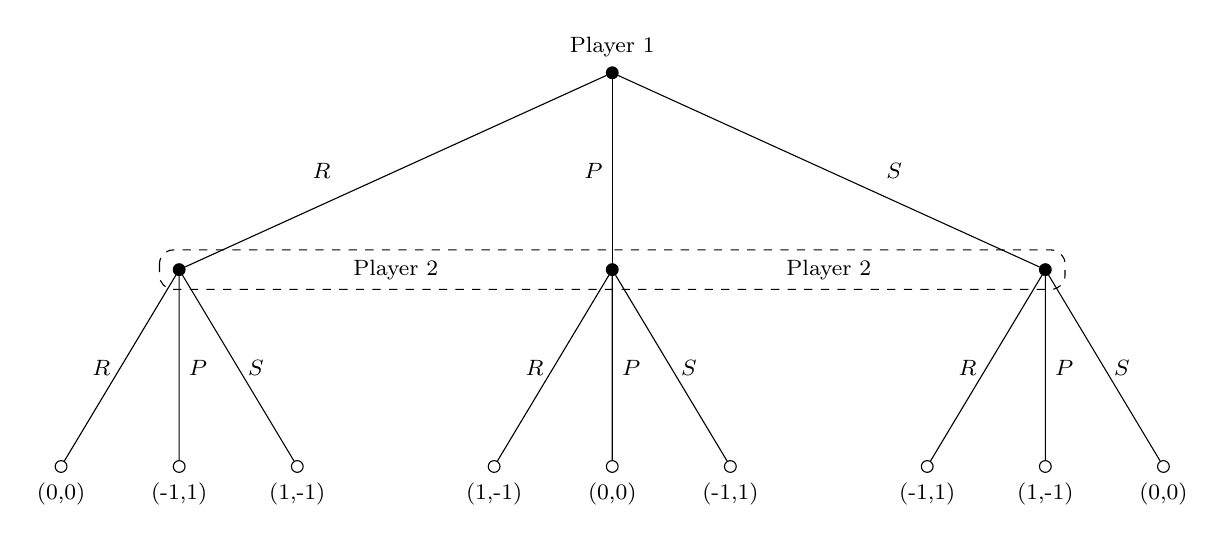
\begin{tikzpicture}[font=\footnotesize]

    \tikzstyle{level 1}=[level distance=25mm, sibling distance=55mm]
    \tikzstyle{level 2}=[level distance=25mm, sibling distance=15mm]

    % Player 1 decision
    \node(0)[solid node, label=above:{Player 1}]{}
        % Player 1 chooses Rock
        child{node(1)[solid node]{}
            %Player 2 Rock
            child{node[hollow node, label=below:{(0,0)}]{} edge from parent node[left]{$R$}}
            %Player 2 Paper
            child{node[hollow node, label=below:{(-1,1)}]{} edge from parent node[right]{$P$}}
            %Player 2 Scissors
            child{node[hollow node, label=below:{(1,-1)}]{} edge from parent node[right]{$S$}}
            edge from parent node[left, xshift=-20]{$R$}
        }
        % Player 1 chooses Paper
        child{node(2)[solid node]{}
            %Player 2 Rock
            child{node[hollow node, label=below:{(1,-1)}]{} edge from parent node[left]{$R$}}
            %Player 2 Paper
            child{node[hollow node, label=below:{(0,0)}]{} edge from parent node[right]{$P$}}
            %Player 2 Scissors
            child{node[hollow node, label=below:{(-1,1)}]{} edge from parent node[right]{$S$}}
            edge from parent node[left]{$P$}
        }
        % Player 1 chooses Scissors
        child{node(3)[solid node]{}
            %Player 2 Rock
            child{node[hollow node, label=below:{(-1,1)}]{} edge from parent node[left]{$R$}}
            %Player 2 Paper
            child{node[hollow node, label=below:{(1,-1)}]{} edge from parent node[right]{$P$}}
            %Player 2 Scissors
            child{node[hollow node, label=below:{(0,0)}]{} edge from parent node[right]{$S$}}
            edge from parent node[left, xshift=30]{$S$}
        }
    ;

    \draw[dashed,rounded corners=5]($(1)+(-.25,.25)$)rectangle($(3)+(.25,-.25)$);

    \node at ($(1)!.5!(2)$) {Player 2};
    \node at ($(2)!.5!(3)$) {Player 2};

\end{tikzpicture}
\end{center}
The `first player' shown in the extensive form does not matter as the other player is inside of an information set since they do not know what the `first player' will pick.
Due to this the order of play has no impact on the outcome of the game.

\section*{Question 3) 2.4 Game Matrix}
Derive the game matrix of the game described in Exercise 4 of Chapter 2.
\begin{center}
\begin{game}{3}{3}[Player 2][Player 1][Rock Paper Scissors]
    &           R                   &               P               &               S               \\
R   &   \phantom{-}0,\phantom{-}0   &   \phantom{-}1,          -1   &             -1,\phantom{-}1   \\
P   &             -1,\phantom{-}1   &   \phantom{-}0,\phantom{-}0   &   \phantom{-}1,          -1   \\
S   &   \phantom{-}1,          -1   &             -1,\phantom{-}1   &   \phantom{-}0,\phantom{-}0   \\
\end{game}
\end{center}

\pagebreak
\section*{Question 4 3.2}
Suppose a manager and a worker interact as follows.
The manager decides whether to hire or not hire the worker.
If the manger does not hire the worker, then the game ends.
When hired the worker chooses to exert either hight effort or low effort.
On observing the worker's effort the manager chooses to retain or fire the worker.
In this game, does "not hire" describe a strategy for the manager? Explain.
\\
\newline
%TODO: Search for this
Check if a strategy has to include trees that cannot be visited.

\section*{Question 5}
Consider the prisoners' dilemma we discussed in class, with the following twist.
If both prisoners choose the same strategy (defect or cooperate) the payoffs are as in the original prisoners' dilemma: when both cooperate each gets a payoff of 2 and if both defect each gets 1. However, if one of them defects and the other cooperates, the one cooperating is given the opportunity to revise his decision. If he does not revise when the payoffs are 3 for the one defecting and 0 for the one cooperating. If he switches ta defect then he gets 1.5 and the other prisoner gets 1.

\begin{enumerate}
\item[(a)] Derive the extensive form of the game.
\item[(b)] Derive the normal for of the game.
\end{enumerate}

\end{document}
